% easychair.tex,v 3.5 2017/03/15

\documentclass{easychair}
%\documentclass[EPiC]{easychair}
%\documentclass[EPiCempty]{easychair}
%\documentclass[debug]{easychair}
%\documentclass[verbose]{easychair}
%\documentclass[notimes]{easychair}
%\documentclass[withtimes]{easychair}
%\documentclass[a4paper]{easychair}
%\documentclass[letterpaper]{easychair}
\usepackage{wrapfig}
\usepackage{doc}
\usepackage{fullpage}
\usepackage{fancyvrb}
\usepackage{amsmath}
\usepackage{amssymb}

% use this if you have a long article and want to create an index
% \usepackage{makeidx}

% In order to save space or manage large tables or figures in a
% landcape-like text, you can use the rotating and pdflscape
% packages. Uncomment the desired from the below.
%
% \usepackage{rotating}
% \usepackage{pdflscape}

% Some of our commands for this guide.
%
\newcommand{\easychair}{\textsf{easychair}}
\newcommand{\miktex}{MiK{\TeX}}
\newcommand{\texniccenter}{{\TeX}nicCenter}
\newcommand{\makefile}{\texttt{Makefile}}
\newcommand{\latexeditor}{LEd}
\def\MC{{\sf MC}}
\def\HB{{\sf HB}}
\def\newterm#1{{\it #1}}

%\makeindex

%% Front Matter
%%
% Regular title as in the article class.
%
\title{Porting the Mathematical Components library to Hierarchy Builder}

% Authors are joined by \and. Their affiliations are given by \inst, which indexes
% into the list defined using \institute
%
\author{
  Reynald Affeldt\inst{3}
  \and
  Xavier Allamigeon\inst{4}
  \and
  Yves Bertot\inst{1}
  \and
  Quentin Canu
  \and
  Cyril Cohen\inst{1}
  \and
  %Marie Kerjean
  %\and
  Pierre Roux
  \and
  Kazuhiko Sakaguchi\inst{2}
  \and
  Enrico Tassi\inst{1}
  \and
  Laurent Th\'ery\inst{1}
  \and
  Anton Trunov
}

% Institutes for affiliations are also joined by \and,
\institute{
  Universit\'e C\^ote d'Azur, Inria, France
\and
   University of Tsukuba, Japan
\and
   AIST, Japan
\and
   Inria, CMAP, CNRS, Ecole Polytechnique, Institut Polytechnique de Paris, France
 }

%  \authorrunning{} has to be set for the shorter version of the authors' names;
% otherwise a warning will be rendered in the running heads. When processed by
% EasyChair, this command is mandatory: a document without \authorrunning
% will be rejected by EasyChair

\authorrunning{The Mathematical Components developers}

% \titlerunning{} has to be set to either the main title or its shorter
% version for the running heads. When processed by
% EasyChair, this command is mandatory: a document without \titlerunning
% will be rejected by EasyChair
\titlerunning{Mathematical Components and Hierarchy Builder}

\begin{document}

\maketitle

% The table of contents below is added for your convenience. Please do not use
% the table of contents if you are preparing your paper for publication in the
% EPiC Series or Kalpa Publications series

%\setcounter{tocdepth}{2}
%{\small
%\tableofcontents}

%\section{To mention}
%
%Processing in EasyChair - number of pages.
%
%Examples of how EasyChair processes papers. Caveats (replacement of EC
%class, errors).

%------------------------------------------------------------------------------
\section{Context}
\label{sect:introduction}

We report on the porting of the Mathematical Components library (hereafter \MC{})
to the Hierarchy Builder~\cite{cohen_et_al:LIPIcs:2020:12356} tool (hereafter \HB{}).

\MC{} is an extensive and coherent repository of formalized
mathematical theories. At the time of writing about 40 opam packages depend
on some components from this library and these packages are not exclusively
focusing on mathematics (e.g., Iris, QuickChick, Disel, \ldots). To our
knowledge about 100 papers about formal proofs build on top of \MC{}.
The library is made of 91 files for a total 124 000 lines of code.

The key to keep the library growing in a rational way is that it revolves
around a hierarchy of interfaces which organizes operations and properties.
Interfaces come with theories which apply, automatically, to all the objects
which are registered as validating the interface. These interfaces are
implemented following the packed classes discipline which works well in practice
but has never been easy to master. Pull Requests extending or \emph{modifying the
hierarchy turned out to be problematic}, hard to review and integrate. Only
a few were merged, the others were put on hold waiting for the library begin
ported to \HB{}.

\begin{wrapfigure}[16]{r}{.40\textwidth}
  \vspace{-1em}
	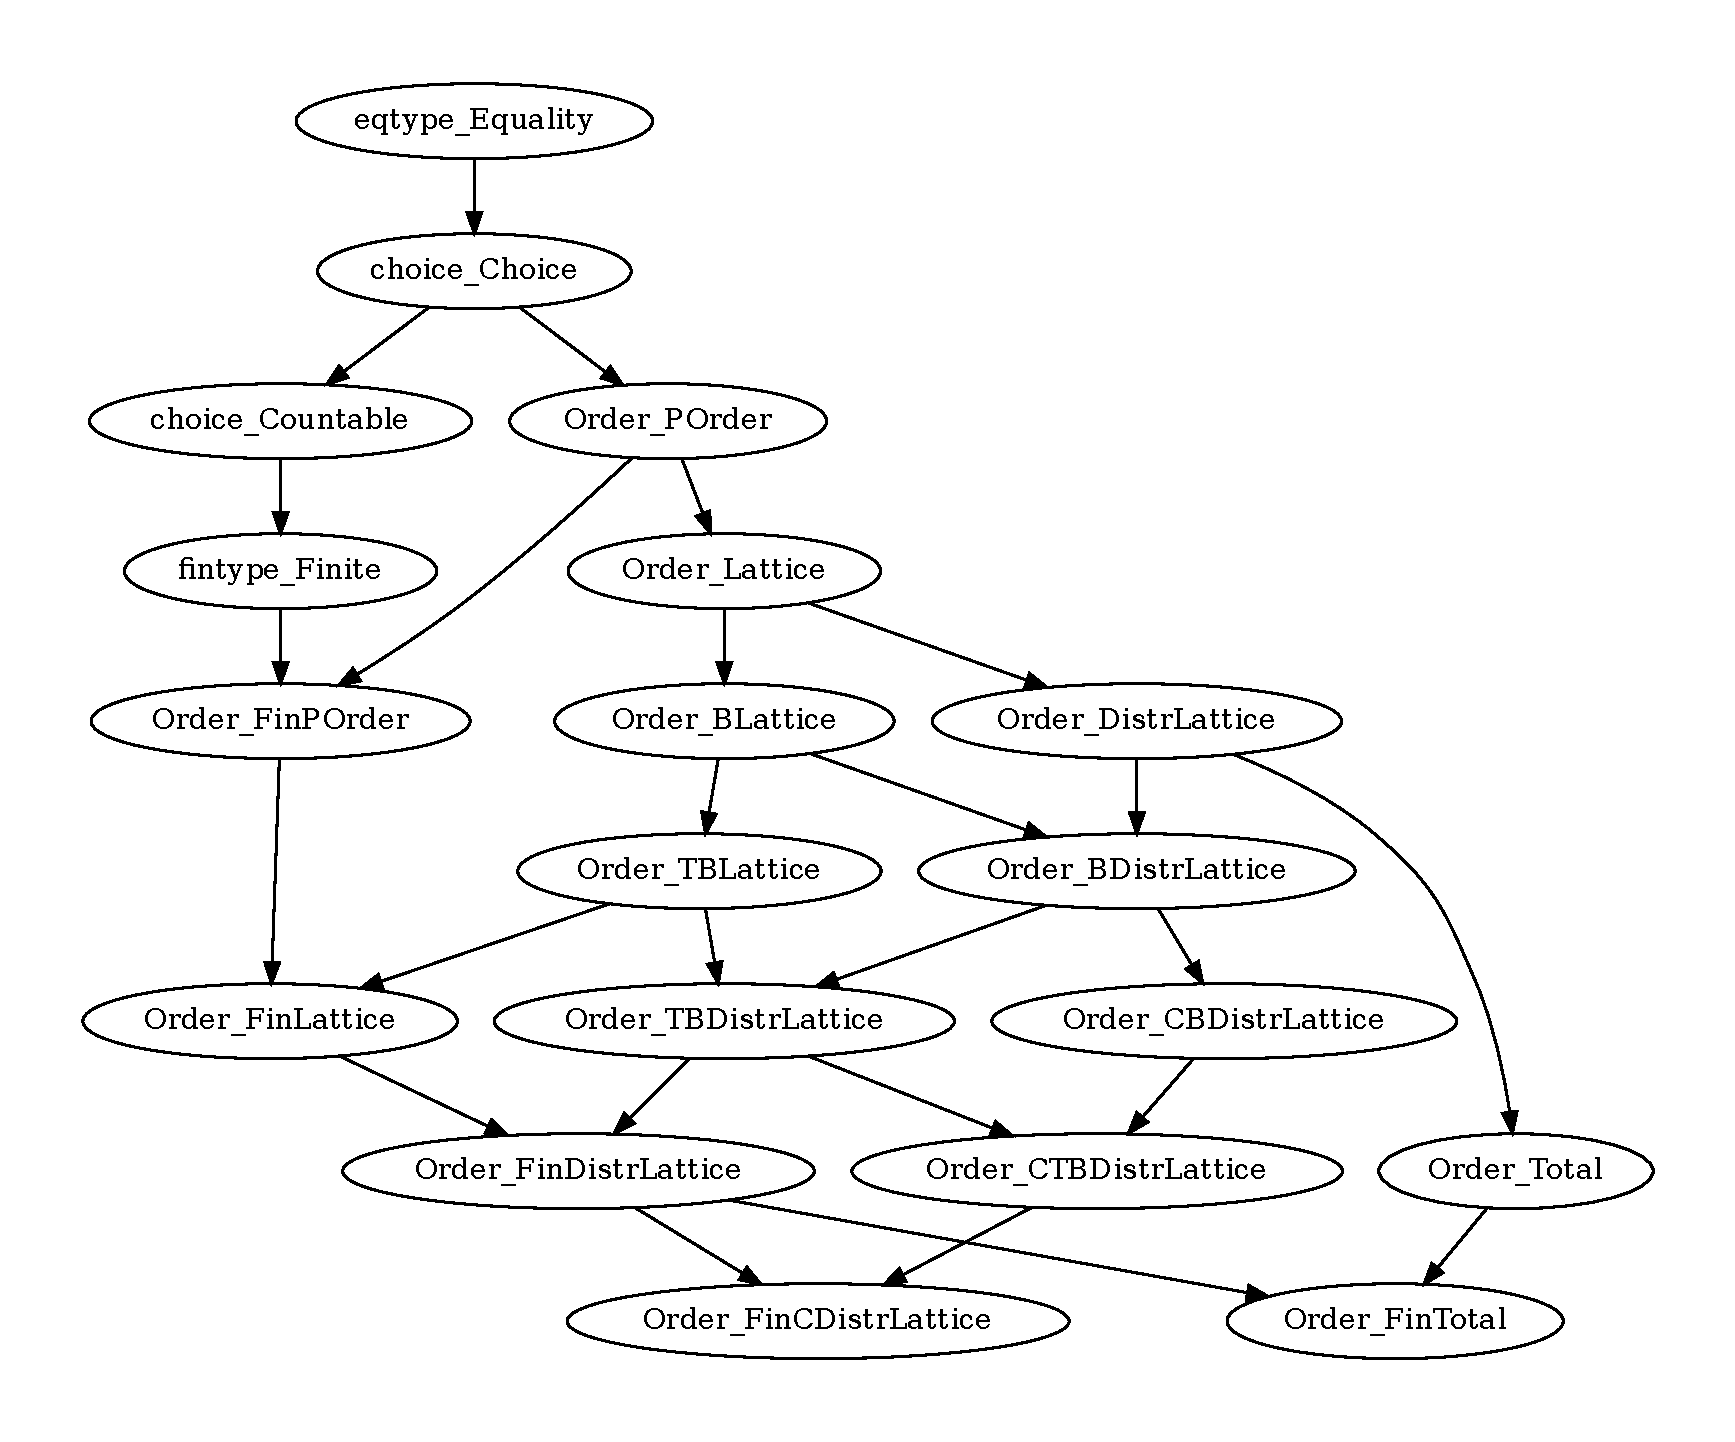
\includegraphics[width=.40\textwidth]{order.pdf}
  \caption{\small Hierarchy in {\tt order.v}}
	\label{fig:order}
  
\end{wrapfigure}
\
\HB{} is a set of high level vernacular commands implemented in Coq-Elpi. It takes
care of automatically synthesizing all the error prone boilerplate required for
packed classed to work. Users just inputs record declarations,
standing for the interfaces, and proofs, for the instances.
They are relieved from
most of the gibberish of modules, sections, coercions, canonical
structures, implicit arguments, phantom abbreviations, \ldots

In the week from the 6th to the 9th of April 2021 the authors of this abstract
gathered (virtually) for a sprint on porting the \MC{} library to
\HB{}. The whole library finally compiled on April 20.
The porting consisted in declaring all the interfaces and their instances
using the new commands, \emph{without changing proofs} in any substantial way.
At the time of writing the patch (\href{https://github.com/math-comp/math-comp/pull/733}{math-comp\#733})
amounts to about 5K lines being edited, and 5K lines being simply \emph{removed}.\\
\
\vspace{-2em}
\section{Report}
\paragraph{Documentation}
\HB{} is a young tool lacking documentation\\
on how to use it proficiently. Some of this knowledge emerged\\
during the sprint and is being archived in the wiki of the project and we
plan to share it with the Coq community at the workshop.[NB(rei): you mean \url{https://github.com/math-comp/hierarchy-builder/wiki}?].

The documentation of the \MC{} library itself is also being reworked, updating
the file header with the new interfaces the user is supposed to used.
In order to ease the documentation effort we extended \HB{} with two commands,
one to draw the hierarchy of interfaces, see~\ref{fig:order} for the excerpt
for the order component, and another one similar to \verb+About+ to access
metadata specific to the the hierarchy, like the known instances of an interface
and where they are declared.
% Thanks to the fact that \HB{} has an internal representation of the hierarchy we could provide a command to
% generate a dot presentation of it, see~\ref{fig:order} for the excerpt for the
% order component, which lost 1300 lines in the process. In addition to that about command to get \HB{}
% specific info.
% 
% \begin{wrapfigure}[12]{r}{.40\textwidth}
% \vspace{-1em}
% \begin{Verbatim}[fontsize=\footnotesize]
%  HB: Order.Total.type is a structure
%      (from "./ssreflect/order.v", line 1588)
%  HB: Order.Total.type characterizing operations
%      and axioms are:
%      - le_total
%  ...
%  HB: Order.Total inherits from:
%      - eqtype.Equality
%      - choice.Choice
%      - Order.POrder
%      - Order.Lattice
%      - Order.DistrLattice
%  HB: Order.Total is inherited by:
%      - Order.FinTotal
% \end{Verbatim}
% \vspace{-1.5em}
% \caption{\small {\tt HB.about.}}
% \label{fig:orderabout}
% \end{wrapfigure}
% 
\paragraph{Performance}

Even if Type Theory lacks a mechanisms to enforce abstraction barriers,
the \MC{} library is built as if one was there: once a new concept is defined
all it's theory is prove (by accessing its definition, and after that the client
is never supposed to unfold the concept. When definitions pile up, unfolding
them can lead to term which are large, too large even for a computer to handle.
In order to prevent performance issues the \MC{} library always ``locked''
some definitions, hiding them behind module signatures.
Since \HB{} uses a more regular but less ``efficient'' representation of
structures we had to lock a few more concepts. Given that the library
was already built with abstraction barriers in mind the changes needed to adapt
proofs (unlocking concepts) were minimal. Moreover we extended \HB{} with
a lock command which takes care of the rather verbose declarations of modules
and theirs signatures.

\paragraph{Instances}

\HB{} provides a built-in concept of \newterm{factory}, a virtual interface which is
compiled to real interfaces automatically. They are mandatory to get backward
compatibility when a library evolves. However, sometimes, defining a factory is
unnecessarily heavy and we prefer to rely on either one or a combination of the
following techniques: we use a lemma which produces a
factory from some (smaller) input; we declare a type alias (identity definition)
which already validates some interfaces and we copy all its instances to a new
type via an automatically generated tool. For example
\verb+Countable.copy T (can_type fgK)+ equips a type \verb+T+ with
\verb+Countable+, \verb+Choice+ and \verb+Equality+ instances proviso a
proof \verb+(fgK : cancel f g)+ where \verb+(f : T -> T')+ and \verb+T'+
is already a \verb+Countable+ type.

\paragraph{Limitations}

The only part of the hierarchy we did not manage to port so far is the
interdependency between normed $\mathbb{Z}$-modules and numeric domains.
Indeed, a normed $\mathbb{Z}$-module is a $\mathbb{Z}$-module on $R$
equipped with a norm with values in a numeric domain $R$,
while a numeric domain is a $\mathbb{Z}$-module on itself, and this apparent
cyclicity which was encodable by hand is not supported by \HB{}.
Since these structures are only really needed in \MC{}-analysis,
we managed to port \MC{} by oversimplifying these structures.
We plan to extend \HB{} to support this kind of self-reference
and enable the porting of \MC{}-analysis.

\paragraph{The scoding sprint}

One of the challenges of the sprint was to contribute simultaneously
to several \MC{} files and eventually update \HB{} with fixed for blocking bugs.
We used a locking mechanism based on Github's check list on the pull request,
whose advancement status was also reflected on the file graph of the library.
Moreover we systematically used a Zulip stream and a Jitsi video chat per file,
allowing the developers to work in little groups, share they progress and
also quickly reach out for help. Using nix to describe the development
environment helped keeping the continuous integration in sync with the
environment used by the developers.
Still, we could have benefit from more tool support. In particular,
an UI that would allow executing in parallel two versions of a Coq script
would have been a plus in this porting activity.

\section{Impact on \MC{} users and perspectives}

The switch to \HB{} leads to \MC{} version 2.0. Updating to it will cause some
breakage but we believe the benefits outweigh the porting burden, if only because
once \HB{} is in place we will be able to rework the hierarchy
\emph{without breaking client code}, since factories can serve as backward
compatible interfaces. Moreover it will trigger a number
of immediate improvements to the library from the addition of new, long awaited,
structures like semilattices and semirings to the integration of existing user
developments (e.g., dioid).
%
Still, given that \MC{} is widely used by the community, we plan to continue
maintaining the 1.x branch even after version 2.0 is officially released
(possibly backporting minor updates which don't require changing the hierarchy).

\label{sect:bib}
\bibliographystyle{plain}
%\bibliographystyle{alpha}
%\bibliographystyle{unsrt}
%\bibliographystyle{abbrv}
\bibliography{bib}

%------------------------------------------------------------------------------


\end{document}

